\documentclass[12pt, a4paper]{report}
\usepackage[utf8]{inputenc} 
%\usepackage[spanish]{babel} 

%% Texto
% Para hipervinculos en las referencias
\usepackage{hyperref}

% Para enumerate con letras
\usepackage[shortlabels]{enumitem}

% [resume]
% https://tex.stackexchange.com/questions/142185/enumeration-across-many-sections
\usepackage{enumitem}

% Para dibujar grafos
\usepackage{tikz}
\usetikzlibrary{positioning, arrows.meta}

% Estilos para dibujar grafos
\tikzset{arco/.style={line width=0.5mm, -latex}}
\tikzset{arista/.style={line width=0.5mm}}
\tikzset{llabel/.style={midway,below,draw=none,fill=none}}
\tikzset{ulabel/.style={midway,above,draw=none,fill=none}}

% Figuras y subfiguras
\usepackage{caption}
\usepackage{subcaption} % subfiguras
\usepackage{float}      % [H] en figuras

%% Simbolos matematicos
\usepackage{amsmath,amsfonts,amssymb,amsthm,epsfig,epstopdf,titling,url,array}
\usepackage{bm} % \bm, https://www.ctan.org/pkg/bm
% \overbrace y \underbrace
\usepackage{mathtools}

\DeclareMathOperator*{\argmax}{argmax}

% Algoritmos
% https://shantoroy.com/latex/how-to-write-algorithm-in-latex/
\usepackage{algorithm}
\usepackage[noend]{algpseudocode} % noend para que no tenga endfor y eso

\usepackage{fullpage}
\usepackage{fancyhdr}

% Imagenes
% https://www.overleaf.com/learn/latex/Inserting_Images
\usepackage{graphicx}

% Teoremas, corolarios, etc.
% https://www.overleaf.com/learn/latex/theorems_and_proofs
\theoremstyle{definition} % Para que no salga en italicas
\newtheorem{theorem}{Teorema}
\newtheorem{lemma}{Lema}
\newtheorem{proposition}{Prop.}

\pagestyle{fancyplain}
\fancyhf{}
\setlength{\headheight}{15pt}

\renewcommand{\headrulewidth}{0pt}

\rhead{Manuel Panichelli}
\chead{1er Parcial AED3: Parte Domiciliaria}
\lhead{L.U. 72/18}
\rfoot{\thepage}

% Distancia del header (\chead) al texto
\setlength{\headsep}{30pt}

\title{1er Parcial AED3: Parte Domiciliaria}
\author{Manuel Panichelli\\L.U. 72/18}
\date{\today}

\begin{document}

\maketitle
\thispagestyle{fancyplain}
\newpage

\chapter*{Preámbulo}

Teoremas, lemas y proposiciones citadas en los ejercicios. La numeración no necesariamente coincide con sus fuentes.

\section*{Grafos}

\begin{proposition}\label{grafos/k_n}
    El grafo completo con $n$ vértices, $K_n$, tiene cantidad de aristas
    \[ m_{K_n} = \frac{n(n-1)}{2}. \]
\end{proposition}

\begin{lemma}\label{grafos/union-caminos}
    La unión de dos caminos simples distintos entre dos vértices contiene un circuito simple.
\end{lemma}

\section*{Arboles}

\begin{theorem}[Definiciones equivalentes de árbol]\label{teo:tree-equiv}
    Dado $G = (V, X)$ un grafo, las siguientes son equivalentes:

    \begin{enumerate}
        \item G es un árbol, un grafo conexo sin circuitos simples.
        \item G es un grafo sin circuitos simples, y $e$ arista tq $e \notin X$,
        el grafo $G + e$ tiene exactamente un circuito simple el cual contiene a
        $e$.\label{teo:tree-equiv-circ}
        \item G es conexo, pero si se saca cualquier arista queda un grafo no
        conexo. Es decir, toda arista es puente.\label{teo:tree-equiv-puentes}

        \item G es un grafo sin circuitos simples y $m=n-1$.
        \item G es conexo y $m=n-1$.\label{teo:tree/equiv/conexo-n-1}
    \end{enumerate}
\end{theorem}

\begin{lemma}\label{lema:tree-g-e}
    Sea $G = (V, X)$ conexo y $e \in X$.

    \[ G - e \ \text{es conexo} \iff \text{e pertenece a un circuito simple de G.} \]
\end{lemma}

\begin{theorem}\label{teo:tree-t-e-f}
    Sean $T = (V, X_T)$ un AG de $G = (V, X)$, $e \in X \setminus X_T$. Luego $T + e - f$ con $f$ una arista del único circuito de $G+e$ es AG de $G$.
\end{theorem}

\begin{theorem}\label{teo:tree/AG}
    Todo arbol conexo tiene al menos un AG.
\end{theorem}

\chapter*{Resolución}

\section*{Ejercicio 1}

\subsection*{Digrafos con forma de $\rho$}
\textit{Un digrafo con loops tiene \textbf{forma de $\bm{\rho}$} cuando todos sus vértices tienen grado de salida igual a 1.}

Antes de comenzar, observo que como el grado de salida de \textbf{todos} los vértices es 1, hay exactamente $n$ arcos ($m = n$)

\begin{enumerate}[a)]
\item \textit{Dibujar 4 digrafos conexos y no isomorfos entre sí que tengan 6 vértices y forma de $\rho$}
    
    Para ello, voy a aprovechar que tienen $m = n$ arcos, y como $n - 1$ es lo mínimo para que sea conexo, basta con ir cambiando el arco redundante para formar diferentes grafos.

    \begin{figure}[H]
        \centering
        \begin{tikzpicture}[
            scale = 1,
            every node/.style={draw,circle,fill=black}
        ]
            \node[] (1) at (0,0) {};
            \node[right=20mm of 1] (2) {};
            \node[right=20mm of 2] (3) {};
            \node[below=20mm of 1] (4) {};
            \node[right=20mm of 4] (5) {};
            \node[right=20mm of 5] (6) {};
        
            \draw[arco] (1) to (2);
            \draw[arco] (2) to (3);
            \draw[arco] (3) to (6);
            \draw[arco] (6) to (5);
            \draw[arco] (5) to (4);
            \draw[arco, dotted] (4) to [loop left] (1);
            \draw[arco, dotted] (4) to [bend right=60] (5);
            \draw[arco, dotted] (4) to (3);
            \draw[arco, dotted] (4) to (1);
        \end{tikzpicture}
        \caption*{Ejemplos de digrafos conexos con forma de $\rho$. Cada arco punteado representa un grafo diferente.}
    \end{figure}

\item \textit{Demostrar que si un digrafo es conexo (cuando su grafo subyacente lo es) y tiene forma de $\rho$ entonces tiene un único ciclo.}

    \begin{proof}[Dem]
    Sea $G$ un digrafo conexo con forma de $\rho$. Su grafo subyacente también será conexo, y por Teo. \ref{teo:tree/AG} tendrá un AG $\bm{T}$, que por Teo. \ref{teo:tree-equiv}.\ref{teo:tree/equiv/conexo-n-1} tiene $m_T = n-1$.

    Como $G$ tiene $m = n$ arcos, sean
    \begin{itemize}
        \item $\bm{G'}$ el sub-digrafo que resulta de convertir devuelta los ejes de T a los arcos de $G$.
        \item $\bm{e = (v, w)}$ el que está demás ($e \notin T, G'$)
    \end{itemize}

    Ya que $T$ es un árbol, no puede tener ciclos, y $G'$ tendrá solo si se juntaron dos arcos de ida y vuelta en uno. Pero en ese caso, $G$ tendría un ciclo, así que voy a suponer que no sucede y que $G'$ no tiene ciclos.

    \begin{figure}[H]
        \centering
        \begin{subfigure}{0.4\textwidth}
            \centering
            \begin{tikzpicture}[
                scale = 1,
                every node/.style={draw,circle,fill=white}
            ]
                \node[](1) at (0,0) {$v$};
                \node[right= 40mm of 1] (2) {$w$};
            
                \draw[arco] (1) to [bend right=60] node[llabel]{$e$} (2); 
                \draw[arco] (2) to [bend right=60] (1);
            \end{tikzpicture}
            \caption*{$G$}
        \end{subfigure}
        \begin{subfigure}{0.4\textwidth}
            \centering
            \begin{tikzpicture}[
                scale = 1,
                every node/.style={draw,circle,fill=white}
            ]
                \node[](1) at (0,0) {$v$};
                \node[right= 40mm of 1] (2) {$w$};
            
                \draw[arista] (1) to [] node[llabel]{} (2); 
            \end{tikzpicture}
            \caption*{$T$ (en este caso igual a $G^s$)}
        \end{subfigure}
        \caption*{Ejemplo de aristas que se combinan}
    \end{figure}

    Como $G'$ no tiene ciclos y si $G$ los tiene, todos los ciclos tienen que contener a $e$. Hay dos casos,

    \begin{itemize}
        \item Si $e$ resulta ser un \textit{loop}, $e = (v, v)$, entonces ese es el ciclo.
        \item Si no, como $e = (v, w)$, $e$ sale de $v$ hacia $w$, y como el grafo es conexo tiene que haber arcos que unan $w$ con $v$, para que en el subyacente haya camino y sea conexo. Además, el camino tiene que estar orientado de $w$ a $v$, ya que si no lo estuviera, los nodos que lo conforman no tendrían grado de salida 1.

        \begin{figure}[H]
            \centering
            \begin{tikzpicture}[
                scale = 1,
                every node/.style={draw,circle,fill=white}
            ]
                \node[](w) at (0,0) {$w$};
                \node[right= 20mm of w] (u) {$u$};
                \node[right= 20mm of u] (v) {$v$};
            
                \draw[arco] (u) to [] node[llabel]{} (w);
                \draw[arco] (u) to [] node[llabel]{} (v);
            \end{tikzpicture}
            \caption*{Ejemplo de digrafo conexo pero que no tiene\\ camino orientado de $w$ a $v$, $d_{OUT}(u) = 2$}
        \end{figure}

        Por lo tanto, se que hay un camino orientado $P$ que va de $w$ a $v$. Y con él puedo armar el ciclo $C: (v, w) + P_{wv}$.

        \begin{figure}[H]
            \centering
            \begin{tikzpicture}[
                scale = 1,
                every node/.style={draw,circle,fill=white}
            ]
                \node[](v) at (0,0) {$v$};
                \node[right= 40mm of 1] (u) {$u$};
                \node[above= 20mm of 2] (w) {$w$};

                \draw[arco] (u) to (v);
                \draw[arco] (w) to (u);
                \draw[arco] (v) to node[ulabel]{$e$} (w);
            \end{tikzpicture}
            \caption*{Ejemplo de ciclo en un digrafo con forma de $\rho$}
        \end{figure}
    \end{itemize}

    Ya se que tiene al menos un ciclo, y este contiene a $e$. Quiero ver que es único. Supongo que no lo es, y que existen dos:
    \begin{align*}
        C_1 &: e + P^1_{vw}\\
        C_2 &: e + P^2_{vw}
    \end{align*}

    Tengo dos caminos distintos de $v$ a $w$ que al no contener a $e$, están también en $T$. En consecuencia su unión también: $P^1_{vw} \cup P^2_{vw} \in T$. Y por Lema. \ref{grafos/union-caminos}, esa unión contiene un circuito simple, que también está en $T$. Pero como T es un árbol, no tiene ciclos. Abs! Entonces el camino es único.

    Concluyo que $G$ tiene un único ciclo.
    \end{proof}

\item \textit{Diseñar un algoritmo para encontrar un ciclo de longitud máxima en un digrafo con forma de $\rho$ (no necesariamente conexo)}

    Para esto, hago un algoritmo iterativo que se fije partiendo de cada nodo si hay un ciclo, y se quede con el de longitud máxima. Supongo que cuento con las funciones

    \begin{itemize}
        \item $\bm{next(v)}$ que dado un vértice $v$, devuelve el único $w$ tal que $(v, w) \in X$, el cual tiene que existir ya que $G$ tiene forma de $\rho$.
        \item Funciones sobre secuencias a lo haskell, cuyas equivalencias en python serian
        \begin{align*}
            \bm{last(s)} &= s[-1] \\
            \bm{head(s)} &= s[0] \\
            \bm{init(s)} &= s[1:] \\
            \bm{length(s)} &= len(s) \\
            \bm{s + w} &= \text{Concatenación}
        \end{align*}
    \end{itemize}

    \algdef{SE}[DOWHILE]{Do}{doWhile}{\algorithmicdo}[1]{\algorithmicwhile\ #1}%
    \begin{algorithm}[H]
        \caption{Algoritmo para encontrar el ciclo con longitud maxima en un digrafo con forma de $\rho$. $O(n \times m)$}
        \label{1/ciclo-max}
        \begin{algorithmic}[1]
            \Function{CicloMax}{$G$}
                \State \textbf{In:} $G = (V, X)$, un digrafo con forma de $\rho$
                \State \textbf{Out:} maxC un ciclo de longitud máxima.
                \State maxC $\gets \langle \rangle$
                \For{$v \in V$}
                    \State C $\gets \langle \rangle$
                    \Do
                        \State C $\gets C + \langle next(last(C)) \rangle$ \Comment{Extiendo el camino}
                    \doWhile{$last(C) \notin init(C)$} \Comment{Mientras no se repita}
                    \If{$last(C) \neq first(C)$} \Comment{Tenemos un subciclo?}
                        \State \textbf{continue} \Comment{Se vera en otra iteración}
                    \EndIf

                    \State maxC $\gets \argmax_{c \in \{C, maxC\}}(length(c))$
                \EndFor

                \State \textbf{return} $maxC$
            \EndFunction
        \end{algorithmic}
    \end{algorithm}

    Para cada vértice, se vé si hay un ciclo partiendo de él extendiendo el camino por el único siguiente. En caso de haberlo, se compara su longitud con el máximo. Hay un chequeo extra para garantizar que no se cuenten erróneamente la longitud de posibles subciclos, ejemplificado en la figura \ref{1/subciclos}. Se ve como al comenzar desde $v$, de no tener ese chequeo, contabilizaríamos a $v\ x\ w\ u\ x$ como un ciclo de longitud errónea.

    \begin{figure}[H]
        \centering
        \begin{tikzpicture}[
            scale = 1,
            every node/.style={draw,circle,fill=white}
        ]
            \node[](v) at (0,0) {$v$};
            \node[right= 20mm of v] (x) {$x$};
            \node[right= 20mm of x] (u) {$u$};
            \node[above= 20mm of u] (w) {$w$};

            \draw[arco] (u) to [] (x);
            \draw[arco] (x) to [] (w);
            \draw[arco] (v) to [] (x);
            \draw[arco] (w) to [] (u);
        \end{tikzpicture}
        \caption{Ejemplo de subciclo en un digrafo con forma de $\rho$}
        \label{1/subciclos}
    \end{figure}

    La complejidad del algoritmo es $O(n \times m)$, ya que el do while interno se ejecuta a lo sumo $m$ veces en total, y el for $n$ veces. Pero como en los digrafos con forma de $\rho$ $n = m$, es $O(n^2)$.

\end{enumerate}

\subsection*{Selección de actividades}

\textit{Período de tiempo circular $[0, T]$, $n$ actividades tal que la $i$-ésima comienza en el instante $s_i$ y termina en $t_i$. Si $s_i > t_i$, la actividad contiene el instante $0=T$. El objetivo es determinar la máxima razón $x / y$ para una secuencia circular de actividades $A_1, \ldots, A_x$ que se realiza en $y$ períodos completos cuando $A_{i+1}$ se inicia lo antes posible una vez terminado $A_i$. Estrategia \textbf{golosa} para elegir actividad $j$ si se eligió $i$: Tomarla como una actividad que no se solapa con $i$ y cuyo tiempo de finalización es el primero desde $t_i$, en un recorrido del tiempo en el sentido de las agujas del reloj. Definir el digrafo de actividades D que tiene un vert $i$ por cada actividad y tiene un arco $i \to j$ cuando $j$ es la elección golosa que se toma si se elige $i$.}

Veamos los ejemplos del enunciado como digrafos y luego lo definimos formalmente
\begin{align*}
    A_0 &= [0, 6]   & A_4 &= [11, 15]\\
    A_1 &= [4, 10]  & A_5 &= [13, 18]\\
    A_2 &= [7, 12]  & A_6 &= [16, 23]\\
    A_3 &= [8, 10]  & A_7 &= [19, 2]
\end{align*}

% \interval{layer}{s}{t}
\newcommand{\interval}[4]{
    \draw (#2, #1) -- (#3, #1) node[ulabel]{#4};
    \draw[fill=white] (#2, #1) circle (0.25);
    \fill (#3, #1) circle (0.25);
}

% para cuando s > t
\newcommand{\loopinterval}[4]{
    \draw (#2, #1) -- (23, #1) node[ulabel]{#4};
    \draw (0, #1) -- (#3, #1) node[ulabel]{#4};
    \draw[fill=white] (#2, #1) circle (0.25);
    \fill (#3, #1) circle (0.25);
}

\begin{figure}[H]
    \centering
    \begin{subfigure}{\textwidth}
        \centering
        \begin{tikzpicture}[scale=0.5]
            % Axis
            \draw (0,0)-- (23,0);
            % Points
            \foreach \x in {0, ..., 23} {
                \draw (\x,0.5) -- (\x,-0.5) node[below] {\x};
            }
            
            \interval{2.5}{0}{6}{$A_0$}
            \interval{2.5}{8}{10}{$A_3$}
            \interval{2.5}{11}{15}{$A_4$}
            \interval{2.5}{16}{23}{$A_6$}
            \interval{1}{4}{10}{$A_1$}
            \loopinterval{1}{19}{2}{$A_7$}
            \interval{4}{13}{18}{$A_5$}
            \interval{4}{7}{12}{$A_2$}
        \end{tikzpicture}
    \end{subfigure}
    \par\bigskip
    \begin{subfigure}{\textwidth}
        \centering
        \begin{tikzpicture}[
            scale = 1,
            every node/.style={draw,circle,fill=white}
        ]
            \node[](0) at (0, 0) {0};
            \node[right=20mm of 1](3) {3};
            \node[below=20mm of 3](4) {4};
            \node[left=20mm of 4](6) {6};
            
            \node[right=10mm of 3](1) {1};
            \node[right=20mm of 1](2) {2};
            \node[right=10mm of 4](5) {5};
            \node[right=20mm of 5](7) {7};
    
            \draw[arco, color=cyan] (0) to [bend left = 30] (3);
            \draw[arco, color=cyan] (3) to (4);
            \draw[arco, color=cyan] (4) to [bend left = 30](6);
            \draw[arco, color=cyan] (6) to (0);

            \draw[arco] (1) to (4);
            \draw[arco] (5) to (7);
            \draw[arco] (2) to (5);
            \draw[arco, dotted] (7) to (1);
            \draw[arco, dotted] (7) to (3);
        \end{tikzpicture}    
    \end{subfigure}
    \caption{Ejemplo de un digrafo de actividades $D$, en \textcolor{cyan}{cyan} el ciclo máximo.}
\end{figure}

Definimos $D = (V, X)$ como
\begin{align*}
    V &= \{ 1, \ldots, x \}\\
    X &= \{ (i, j) \mid i \in V, \text{noSeSolapan}(i, j) \wedge \text{terminaAntes}(i, j, k)\ \forall k\}
\end{align*}

Donde
\begin{itemize}
    \item noSeSolapan(i, j) es verdadero sii las actividades $A_i$ y $A_j$ no se solapan.
    \item terminaAntes(i, j, k) es verdadero si la actividad $A_j$ tiene un tiempo de finalización anterior a $A_k$ a partir del de $A_i$, en un recorrido del tiempo en el sentido de las agujas del reloj. En caso de empate, prefiere la de menor número.
\end{itemize}

\begin{enumerate}[a), resume]
\item Intuitivamente, como es un arbol de elecciones de un algoritmo goloso, tiene sentido que tenga forma de $\rho$ ya que desde cada nodo se hará una sola elección que nunca se revise. Viendo la definición formal, efectivamente para cada vertice (actividad) elegimos una sola: la que termine primero. Por lo tanto, para cada $i\ \exists!\ j : (i, j) \in X$. Entonces el grado de salida de todo vertice $i$ es 1, y el grafo $D$ tiene forma de $\rho$.

\item \textit{Demostrar que el ciclo máximo de D es una solución al problema de selección de actividades.}

opcional, no lo hago

\item \textit{Dar un algoritmo para resolver el problema de selección de actividades, suponiendo que se describen usando un conjunto de pares $[s_i, t_i]$ con $0 \leq s_i, t_i \leq T, s_i \neq t_i$ y $T = 2n$}

    Describo los pasos que tomaría el algoritmo en lenguaje coloquial. Este debe, dada una lista de actividades, devolver la máxima razón $x / y$ para una secuencia circular de actividades $A_1, \ldots A_x$ que se realiza en $y$ períodos completos.

    \begin{enumerate}[1.]
        \item Armo el digrafo D con las tareas como vértices, y para cada una aplico el algoritmo goloso para conseguir a cual hacerlo adyacente. La complejidad del algoritmo goloso es $O(n^2)$, pues para cada actividad se ven todas las demás para ver cual tiene el tiempo de finalización mas corto. Entonces la complejidad total de este paso es $O(n^3)$.
        \item Como el ciclo máximo de $D$ es la secuencia circular, y $D$ es un digrafo con forma de $\rho$, puedo usar el algoritmo \ref{1/ciclo-max} para encontrarlo. Lo llamo $C$, y luego $x = length(C)$. Este paso se ejecuta en $O(n^2)$
        \item Falta encontrar $y$, que es la cantidad de períodos que toma realizar las actividades del ciclo $C$. Para ello, recorro el ciclo, y si el inicio de la actividad $i$ es anterior a la finalización de la $i-1$, incremento la cantidad de períodos. Como se recorre el ciclo que tiene a lo sumo $m = n$ aristas, este paso se ejecuta en $O(n^2)$.
        \item Devuelvo la máxima razón: $x / y$.
    \end{enumerate}

    Finalmente, la complejidad temporal del algoritmo será $O(n^3)$.

\end{enumerate}

\newpage
\section*{Ejercicio 2}

\textit{Hilera con n recipientes con $r_1, \ldots, r_n \in \mathbb{N}$ unidades de agua, se quiere traspasar a dos baldes con capacidades $B_1, B_2 \in \mathbb{N}$. En cada paso se toma el primer recipiente de la hilera y se vuelva completamente en uno de los baldes. Se repite mientras algun balde tenga capacidad suficiente para albergar \textbf{toda} el agua del recipiente. El objetivo es maximizar la cantidad de recipientes que se vuelcan.}

\begin{enumerate}[a)]
    \item Formulo de forma recursiva una solución del problema con una función matemática $f(i, b)$ la cual tendrá la siguiente semántica: $f(i, b)$ es la máxima cantidad de recipientes que se pueden volcar suponiendo que ya se volcaron $r_1, ... r_{i-1}$ y que el balde con capacidad $B_1$ tiene $b$ de capacidad restante. Observo que esta información es suficiente para inferir la capacidad restante del balde $B_2$, dada por 
    
    \[ 
        b_2 = B_2 -
            \overbrace{
            \underbrace{\sum_{j=1}^{i-1} r_j}_{\substack{\text{total}\\\text{volcado}}} - 
            \underbrace{(B_1 - b).}_{\text{volcado en} \ B_1}
            }^{\text{volcado en} \ B_2}
    \]

    Veamos la función recursiva:

    \[ 
        f(i, b) =
            \begin{cases}
                0 & \text{si} \ (r_i > b \ \text{y}\  r_i > b_2) \ \text{o} \ i = n+1 \\
                f(i+1,\ b) + 1 &\text{si}\ r_i > b\\
                f(i+1,\ b - r_i) + 1 &\text{si}\ r_i > b_2\\
                max\{f(i+1, b),\ f(i+1,\ b - r_i)\} + 1 &\text{si no}
            \end{cases}
    \]

    Explicada en palabras,

    \begin{itemize}
        \item Si $(r_i > b \ \text{y}\  r_i > b_2)$, ninguno de los dos baldes tiene capacidad suficiente para albergar el contenido del recipiente $i$-ésimo. Como no se pueden saltear, terminamos.
        \item Si $i = n + 1$, ya consideramos todos los recipientes.
        \item Si no entra en $B_1$ continuamos por $B_2$, y viceversa.
        \item Si entra en ambos, tomamos ambos caminos y devolvemos el mejor.
    \end{itemize}

    \item Es fácil ver que tiene la propiedad de \textit{superposición de subproblemas}, basta con que alguna cantidad de recipientes sumen lo mismo, y así volcarlos en cada balde sería indistinto y llevaría al mismo resultado. Por ejemplo, cuando más de un recipiente tiene la misma cantidad de agua. Sean $r_1 = r_2 = 5, r_3 = 10$ y $B_1 = B_2 = 20$.
    
    % https://texample.net/tikz/examples/tree/
    \begin{figure}[H]
        \centering
        \begin{tikzpicture}[
            every node/.style = {
                shape=rectangle, rounded corners,
                draw, align=center,
                top color=white
            }
        ]
        \tikzstyle{level 1}=[sibling distance=60mm] 
        \tikzstyle{level 2}=[sibling distance=40mm] 
        \tikzstyle{level 3}=[sibling distance=30mm]
        \tikzstyle{level 3}=[sibling distance=20mm]

            \node{f(1, 20)}
                child { 
                    node{f(2, 15)}
                        child {
                            node{f(3, 10)}
                                child{node{f(4, 0)}}
                                child{node[color=red]{f(4, 10)}}
                        }
                        child {
                            node[color=red]{f(3, 15)}
                                child{node{f(4, 5)}}
                                child{node{f(4, 15)}}
                        }
                }
                child { 
                    node{f(2, 20)}
                        child {
                            node[color=red]{f(3, 15)}
                        }
                        child {
                            node{f(3, 20)}
                                child{node[color=red]{f(4, 10)}}
                                child{node{f(4, 20)}}
                        }
                };
        \end{tikzpicture}
        \caption{Ejemplo de superposoción de subproblemas. En rojo las llamadas que se superponen.}
    \end{figure}

    \item A continuación un algoritmo de programación dinámica \textit{top-down} que implementa la función recursiva de forma bastante directa, agregando memoización mediante una matriz $M$ de $n \times B_1$, cuyo valor por defecto es -1. Suponiendo que $B_1, B_2$, los $r_i$ y $M$ son globales,
    
    % http://tug.ctan.org/macros/latex/contrib/algorithmicx/algorithmicx.pdf
    \begin{algorithm}[H]
        \caption{Implementación con programación dinámica.}
        \begin{algorithmic}[1]
            \Function{Baldes}{$i,\ b$}
                \State $b_2\gets B_2 - \sum_{j=1}^{i-1} r_j - (B_1 - b)$ \Comment{$O(n)$}
                \If{$i = n+1$ o ($r_i > b$ y $r_i > b_2$)}
                    \State \textbf{return} 0
                \EndIf

                \If{$M[i][b] = -1$} \Comment{No está memoizado}
                    \If{$r_i > b$}
                        \State $M[i][b] \gets Baldes(i + 1, b) + 1$
                    \ElsIf{$r_i > b_2$}
                        \State $M[i][b] \gets Baldes(i + 1, b - r_i) + 1$
                    \Else
                        \State $M[i][b] \gets max\{Baldes(i+1, b),\ Baldes(i+1, b - r_i)\} + 1$
                    \EndIf
                \EndIf

                \State \textbf{return} $M[i][b]$
            \EndFunction
        \end{algorithmic}
    \end{algorithm}
    
    El problema se resuelve con el llamado $Baldes(0,\ B_1)$

    \item La complejidad temporal del algoritmo \textit{top-down} es igual a cualquier otro algoritmo de PD, (\#subproblemas $\times$ costo de cada subproblema). En este caso, la cantidad de subproblemas es $n \times B_1$, y cada uno se resuelve en $O(n)$ (cálculo de $b_2$ y el resto operaciones en tiempo constante). Por lo tanto la complejidad es $O((n \times B_1) \times n) = O(n^2 \times B_1)$. Noto que esto podria mejorarse a $O(n \times B_1)$ evitando calcular $b_2$ en cada llamado, incrementandolo de a 1 en cada llamado.
        
\end{enumerate}

\newpage
\section*{Ejercicio 3}

\begin{enumerate}[a)]
    \item La imagen muestra un ejemplo de por qué las \textit{social bubbles} no funcionan. Uno cree que está en una burbuja pequeña, con solo la gente con la que se ve, pero en realidad la burbuja se extiende con la burbuja de cada individuo. De esa forma, termina siendo mucho más grande de lo esperado.
    
    Visto como grafos, cada persona sería un vértice, y dos personas son adyacentes entre sí si tuvieron contactos estrechos. Las burbujas sociales pasarían a ser componentes conexas, y uno cree que está en una componente conexa chica pero en realidad se extiende por los vecinos de cada nodo, y termina siendo un grafo conexo. Cada contagio que se produzca en cualquier lado termina llegando a su burbuja.

    \item \textit{Probar que un grafo de $n$ vértices que tiene más de $((n-1)(n-2))/2$ aristas es conexo.}
    
    qvq si $m > \frac{(n-1)(n-2)}{2}$ entonces G cualquiera es conexo. Lo voy a probar haciendo uso del siguiente lema.

    \begin{lemma}\label{3/lemma}
        Sea G un grafo cualquiera,
        \[
            m = \frac{(n-1)(n-2)}{2} 
            \implies 
            G \text{ es conexo o es } K_1 + K_{n-1} \\
        \]
    \end{lemma}

    \begin{proof}[Dem (Lema \ref{3/lemma})]
        Veamos con más detalle cómo se puede interpretar la fórmula
        % https://tex.stackexchange.com/questions/36153/annotating-individual-math-terms-with-braces/36154
        \[
            m = \frac
            {
                \overbrace{(n-1)}^{\mathclap{\substack{\text{Todos los nodos}\\\text{menos 1}}}}
                \quad
                \times
                \quad
                \overbrace{(n-2)}^{\mathclap{\substack{\text{Conectan con todo}\\\text{el resto menos 1}}}}
            }
            {
                \underbrace{2}_{\mathclap{\text{Porque son pares no ordenados}}}
            }.
        \]

        Por lo tanto, puedo construir iterativamente a cualquier grafo que tenga esta cantidad de ejes conectandolo a $(n - 1)$ nodos con todos menos 1. Por ejemplo,

        \begin{figure}[H]
            \centering
            \begin{subfigure}{0.4\textwidth}
                \centering
                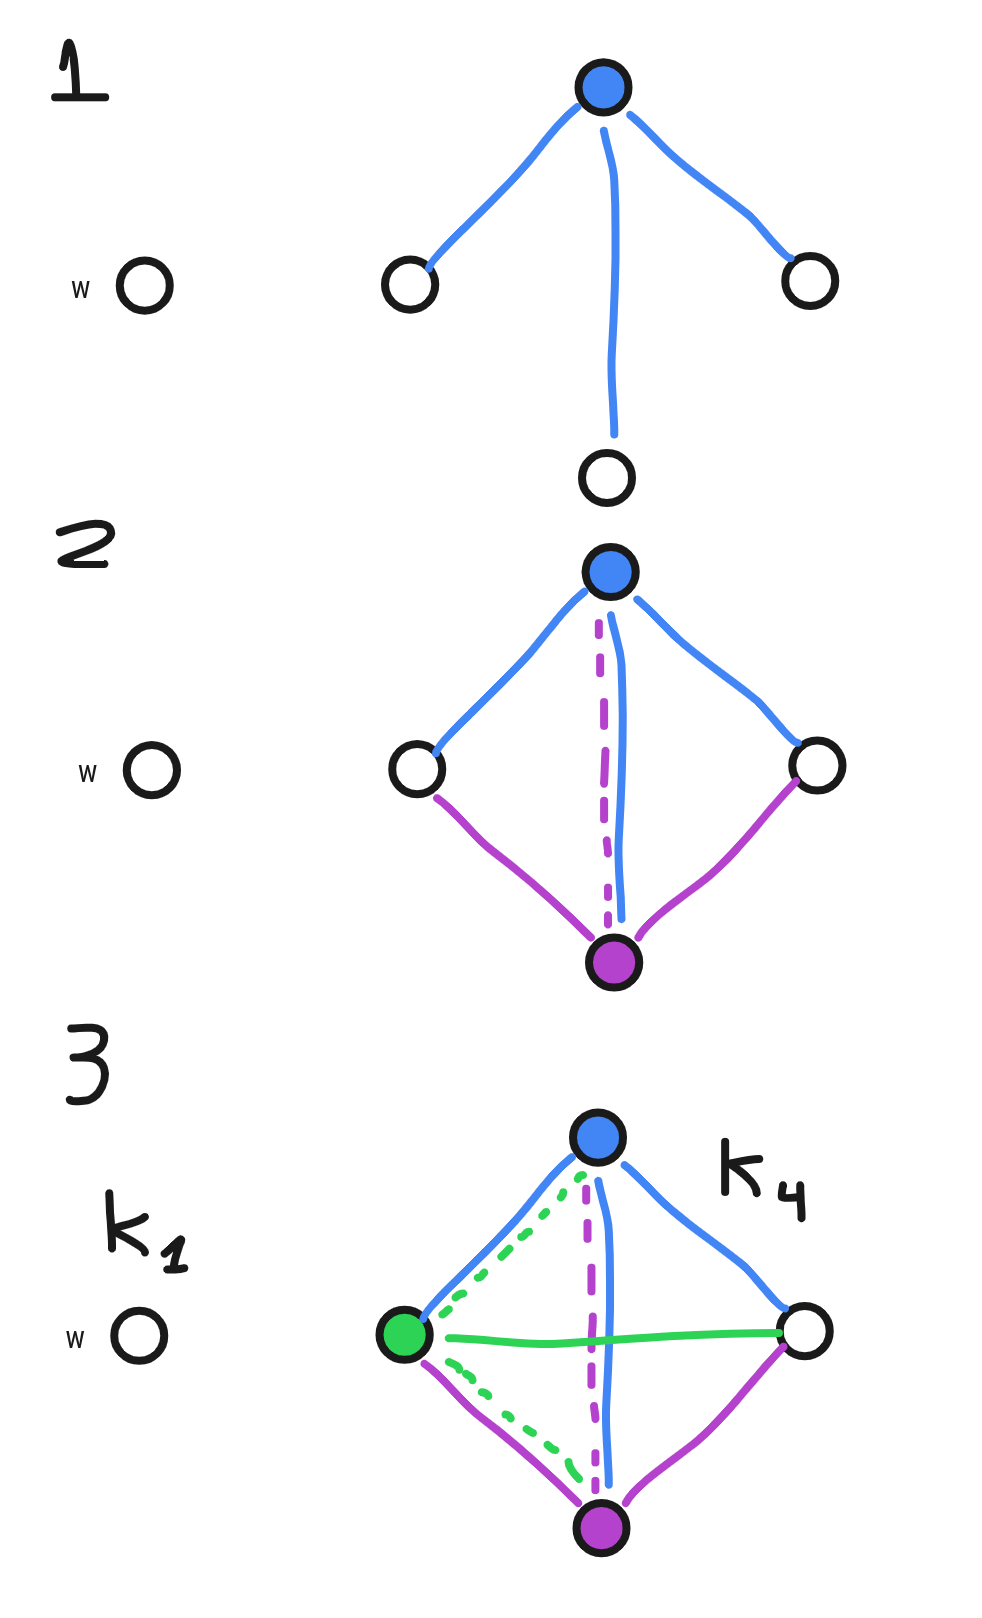
\includegraphics[scale=0.15]{img/3-k1-kn-1.png}
                \caption{Ejemplo de construcción que lleva a $K_1 + K_{n-1}$}
            \end{subfigure}
            \qquad
            \begin{subfigure}{0.4\textwidth}
                \centering
                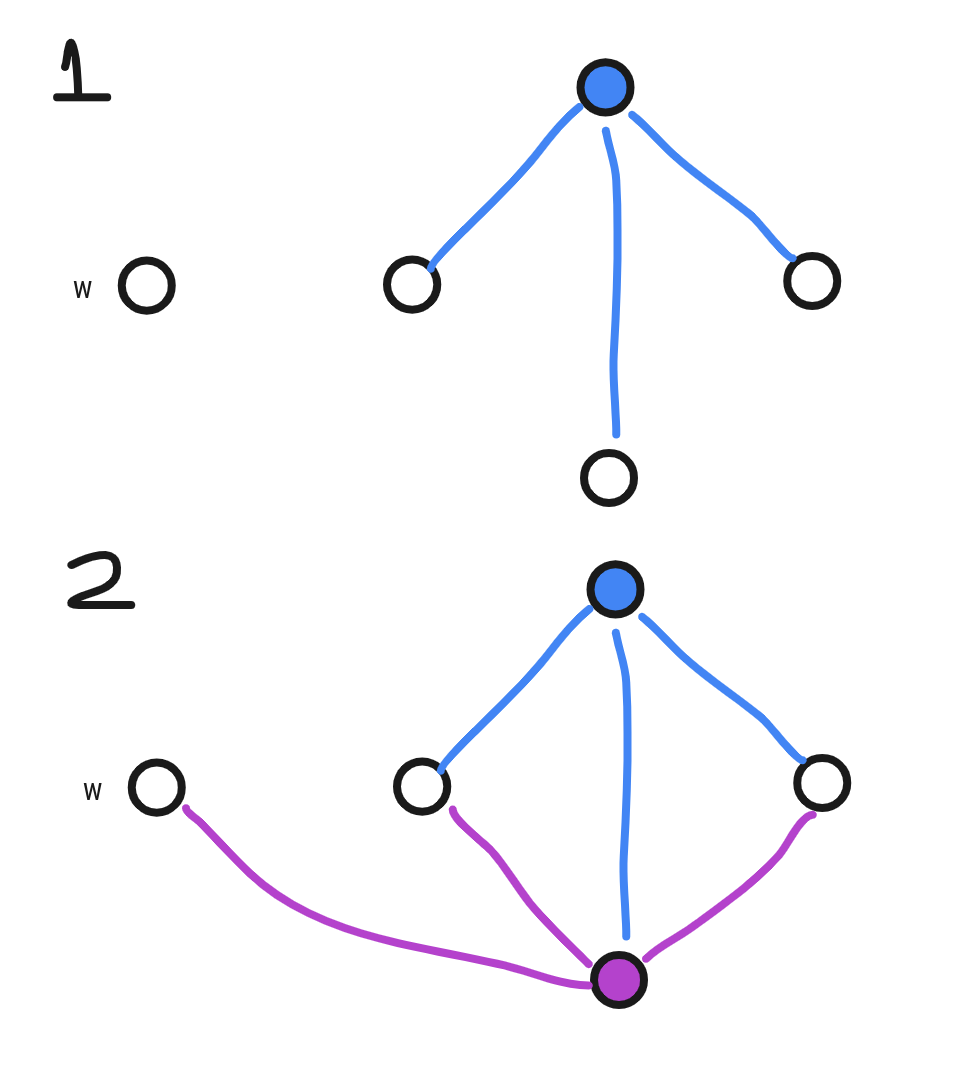
\includegraphics[scale=0.15]{img/3-conexo.png}
                \caption{Ejemplo de construcción que lleva a un grafo conexo}
            \end{subfigure}
            \caption{Algunos grafos posibles para $n = 5, m = 6$}
        \end{figure}

        Y para grafos generales, para cada nodo $v_i \in V \setminus \{w\}$ con $w \in V$ cualquiera,

        \begin{itemize}
            \item Para el primero, lo conecto con todos los nodos excepto uno, $w$. De esta manera quedan definidas dos componentes conexas, $w$ y el resto de los nodos.
            \item Para el segundo, tengo dos opciones. Puedo conectarlo con $w$ y todos menos 1 de $V \setminus \{w\}$, con lo cuál quedaría conexo, ya que ellos ya estaban conectados a través de $v_1$, o puedo conectarlo con todos los nodos de $V \setminus \{w\}$ y así seguir dejando a $w$ aislado.
            \item Sigo así hasta el último de $V \setminus \{w\}$, si lo conecto con $w$ quedaría G conexo, y sino queda partido en dos: $w$ por un lado, y $K_{n-1}$ por el otro, ya que cada nodo estaba conectado con todos menos $w$, formando así un subgrafo completo.
        \end{itemize}
    \end{proof}

    Ahora si, demuestro el ejercicio pedido
    \begin{proof}[Dem (3b)]
        Ya que $m > \frac{(n-1)(n-2)}{2}$, se agrega al menos una arista a $G'$, el subgrafo de $G$ que tiene exactamente $m = \frac{(n-1)(n-2)}{2}$. Por \eqref{3/lemma}, $G'$ es conexa o tiene dos componentes conexas, $K_1$ y $K_{n-2}$.
        
        \begin{itemize}
            \item Si $G'$ es conexa, agregar solo aristas a un grafo conexo seguirá siendo conexo.
            \item Sino, $G' = K_1 + K_{n-2}$, y las aristas que se agregan no pueden ir dentro de cada componente conexa, ya que son grafos completos. Necesariamente tienen que tener un extremo en cada una. Al unirse las componentes conexas, $G$ queda conexo.
        \end{itemize}

        Para ambos casos $G$ es conexo.
    \end{proof}
    
\end{enumerate}

\newpage
\section*{Ejercicio 4}

\textit{Un \textbf{puente} de un grafo es un eje del grafo tal que al removerlo
se obtiene un grafo con más c.cs. Sea $G = (V, X)$ un grafo conexo y $e \in X$.
Demostrar que e es un puente de G sii e pertenece a todo AG de G.}

\begin{proof}[Dem]
    Veamos la ida y la vuelta.

    \begin{enumerate}
        \item[$\Rightarrow$)] Sea $e$ puente de G. qvq pertenece a todo AG de G.
         
        Voy a probar el contrarecíproco, $e \notin T$ un AG de G $\implies$ $e$ no es puente de G
        \begin{align*}
            e \notin T &\implies T+e\ \text{tiene un ciclo C que contiene a e} & \text{(Teo. \ref{teo:tree-equiv}.\ref{teo:tree-equiv-circ}, $T$ árbol)}\\
            &\implies C \in G &(C \in T+e \subseteq G)\\
            &\implies e \text{ pertenece a un ciclo de G}\\
            &\implies G - e \text{ es conexo} &\text{(Lema \ref{lema:tree-g-e})}\\
            &\implies G - e \text{ \textbf{no} tiene menos componentes conexas que G}\\
            &\implies e \text{ \textbf{no} es puente de G.} &\text{(por def de puente)}
        \end{align*}

        \item[$\Leftarrow$)] qvq $e$ pertenece a todo AG de G $\implies$ $e$ es puente de G.

        Se que $e$ es puente $\iff G - e$ tiene más componentes conexas que G. Y si G es conexo, eso quiere decir que $G - e$ no lo es. Supongo que no es puente y que $e = (v, w)$.
        \begin{align*}
            e\ \text{no es puente} &\implies G - e\ \text{es conexo}    & (\text{G conexo})\\
            &\implies e \in C\ \text{un circuito simple de G,} & (\text{por Lema \ref{lema:tree-g-e}})
        \end{align*}
        y lo descompongo de la siguiente manera,

        \begin{figure}[H]
            \centering
            \begin{tikzpicture}[
                scale = 1,
                every node/.style={draw,circle,fill=white}
            ]
                \node[](v) at (0,0) {$v$};
                \node[right= 40mm of v] (w) {$w$};
    
                \draw[arista, color=orange] (v) to [] node[ulabel]{$e$} (w);
                \draw[arista] (w) to [bend left = 60] node[llabel]{$P_{vw}$}(v);
            \end{tikzpicture}
            \caption*{$C: e + P_{vw}$}
        \end{figure}

        Como hay dos caminos para ir de $v$ a $w$, voy a tener al menos dos AG distintos, uno para cada camino. Sea $T$ el que contiene a $P_{vw}$. Como $e$ pertenece a todo AG, en particular $e \in T$. Pero como $P_{vw} \in T \wedge e \in T \implies C: e + P_{vw} \in T$. Abs! $T$ es un arbol, no puede tener circuitos. Como el absurdo provino de suponer que $e$ no era puente de G, concluyo que sí lo es, que es lo que quería probar.

    \end{enumerate}

\end{proof}

\newpage
\section*{Ejercicio 5}

\textit{Cabinas de peaje inverso, en las que se le paga un monto al conductor que pase. Cada cabina de peaje $i \in \{1 \dotso C \}$ tiene un costo asociado $c_i$, el cual es negativo para las cabinas inversas, y el costo $c_{ij}$ del viaje de la cabina $i$ a la $j$, en caso de que se pueda de forma directa.}

\begin{enumerate}[a)]
\item Para modelar el problema, me gustaría representar a las cabinas como nodos, donde una cabina es adyacente a otra si se puede viajar de forma directa. Pero tenemos un problema, las aristas y los vértices tendrían peso, cuando los grafos que modelamos solo tienen peso en las aristas. Vamos a tener que usar una representación muy similar a la de la clase de Mirko\footnote{\url{https://campus.exactas.uba.ar/pluginfile.php/232068/mod\_resource/content/1/CAMINOS\%20MINIMOS.pdf}}.
Veamos un ejemplo

\begin{figure}[H]
    \centering
    \begin{subfigure}[b]{0.4\textwidth}
        \centering
        \begin{tikzpicture}[scale = 1,every node/.style={draw,circle,fill=white}]
            % La sintaxis es \node[opciones] (nombre del nodo) {dentro};    
            \node[label={1}](1) at (0,0) {$c_1$};
            \node[label={2},right= 40mm of 1] (2) {$c_2$};
        
            \draw[line width=0.5mm,-latex] (1) to node[midway,below,draw=none,fill=none]{$c_{12}$} (2); 
            \draw[line width=0.5mm,-latex] (2) to [bend right=60] node[midway,above,draw=none,fill=none]{$c_{21}$} (1);
        \end{tikzpicture}
        \caption{Digrafo original}
    \end{subfigure}
    \begin{subfigure}[b]{0.4\textwidth}
        \centering
        \begin{tikzpicture}[scale = 1,every node/.style={draw,circle,fill=white}]
            % La sintaxis es \node[opciones] (nombre del nodo) {dentro};    
            \node[label={$1_a$}](1a) at (0,0) {};
            \node[label={$1_b$}, right=10mm of 1a](1b) {};

            \node[label={$2_a$},right= 20mm of 1b] (2a) {};
            \node[label={$2_b$},right= 10mm of 2a] (2b) {};

            \draw[line width=0.5mm,-latex] (1a) to node[midway,below,draw=none,fill=none]{$c_{1}$} (1b);
            \draw[line width=0.5mm,-latex] (2a) to node[midway,below,draw=none,fill=none]{$c_{2}$} (2b);

            \draw[line width=0.5mm,-latex] (1b) to node[midway,below,draw=none,fill=none]{$c_{12}$} (2a); 
            \draw[line width=0.5mm,-latex] (2b) to [bend right=60] node[midway,above,draw=none,fill=none]{$c_{21}$} (1a);
        \end{tikzpicture}
        \caption{Digrafo adaptado}
    \end{subfigure}
    \caption{Ejemplo de representación de cabinas con digrafos}
    \label{5:adaptado}
\end{figure}

Separo cada nodo $i$ con peso $c_i$ en dos, $i_a$ e $i_b$, con un arco de peso $c_i$ de $i_a$ a $i_b$. Todos los arcos salen de $i_b$, y llegan a $i_a$. De esta forma, me aseguro que cualquier camino que pase por el nodo pague el costo del peaje. Luego, habrá un arco de $i_b$ a $j_a$ con peso $c_{ij}$ si es posible viajar de forma directa de la cabina $i$ a la $j$.

Matemáticamente, $G = (V, X)$ donde
\begin{align*}
    V = \ &\{ 1_a, 1_b, \ldots C_a, C_b\},\\
    X = \ &\{ (i_b, j_a, c_{ij}) \mid \text{se puede viajar de forma directa de i a j} \}\ \cup\\
      &\{ (i_a, i_b, c_i) \mid i \in \{1, \ldots, C\}\}.
\end{align*}

Con este modelo, se podrá obtener una ganancia recorriendo \textit{eternamente} las cabinas si el grafo tiene \textbf{ciclos negativos}, circuitos que luego de recorrerlos dan una ganancia.

\begin{figure}[H]
    \centering
    \begin{subfigure}[b]{0.4\textwidth}
        \centering
        \begin{tikzpicture}[scale = 1,every node/.style={draw,circle,fill=white}]
            % La sintaxis es \node[opciones] (nombre del nodo) {dentro};    
            \node[label={$1_a$}](1a) at (0,0) {};
            \node[label={$1_b$}, right=10mm of 1a](1b) {};

            \node[label={$2_a$},right= 20mm of 1b] (2a) {};
            \node[label={$2_b$},right= 10mm of 2a] (2b) {};

            \draw[line width=0.5mm,-latex] (1a) to node[midway,below,draw=none,fill=none]{-10} (1b);
            \draw[line width=0.5mm,-latex] (2a) to node[midway,below,draw=none,fill=none]{-5} (2b);

            \draw[line width=0.5mm,-latex] (1b) to node[midway,below,draw=none,fill=none]{5} (2a); 
            \draw[line width=0.5mm,-latex] (2b) to [bend right=60] node[midway,above,draw=none,fill=none]{10} (1a);
        \end{tikzpicture}
        \caption{Cabinas sin ciclos negativos}
        \label{5/ej/sin}
    \end{subfigure}
    \begin{subfigure}[b]{0.4\textwidth}
        \centering
        \begin{tikzpicture}[scale = 1,every node/.style={draw,circle,fill=white}]
            % La sintaxis es \node[opciones] (nombre del nodo) {dentro};    
            \node[label={$1_a$}](1a) at (0,0) {};
            \node[label={$1_b$}, right=10mm of 1a](1b) {};

            \node[label={$2_a$},right= 20mm of 1b] (2a) {};
            \node[label={$2_b$},right= 10mm of 2a] (2b) {};

            \draw[line width=0.5mm,-latex] (1a) to node[midway,below,draw=none,fill=none]{-10} (1b);
            \draw[line width=0.5mm,-latex] (2a) to node[midway,below,draw=none,fill=none]{-5} (2b);

            \draw[line width=0.5mm,-latex] (1b) to node[midway,below,draw=none,fill=none]{5} (2a); 
            \draw[line width=0.5mm,-latex] (2b) to [bend right=60] node[midway,above,draw=none,fill=none]{\textbf{5}} (1a);
        \end{tikzpicture}
        \caption{Cabinas con ciclos negativos}
        \label{5/ej/con}
    \end{subfigure}
    \caption{Ejemplo de cabinas con y sin ciclos negativos}
    \label{5/ej}
\end{figure}

En la figura \ref{5/ej} se pueden ver dos ejemplos de cabinas y montos. En \ref{5/ej/sin} no hay ningún ciclo negativo, a pesar de que el camino $P: 1_a\ 1_b \ 2_a \ 2_b$ tiene costo -10, al volver a $1_a$ se vuelve 0, con lo cual recorrer infinitamente nunca daría ganancias. En cambio, en \ref{5/ej/con} se puede ver como con un pequeño ajuste, el ciclo $C: 1_a\ 1_b \ 2_a \ 2_b \ 1_a$ tiene costo -5, con lo cual se puede recorrer eternamente, generando ganancias.

\item Para resolver el problema del inciso anterior, basta con ver si hay ciclos negativos en algún camino de una cabina a la otra. Para ello, se puede usar el algoritmo de \textbf{Floyd}, pensado para resolver camino mínimo \textit{múltiples orígenes, múltiples destinos}, que puede ser adaptado para detectar ciclos negativos. Este tiene una complejidad temporal de $O(n^3)$ con $n$ la cantidad de vertices. Y en nuestro caso, $n = 2 \times|C|$, el doble de la cantidad de cabinas, ya que cada una se separa en dos nodos.

\end{enumerate}
\end{document}